\section{Ethan}

\subsection{Aufgabenstellung}

\begin{enumerate}
    \item Energie in Abhängigkeit des Diederwinkels zeichnen und die Anzahl der Min- bzw. Maxima bestimmen.
    \item Auswertung der erhaltenen Werte.
    \item Statistische Fehlerrechnung
    \item Vergleich der Methoden 
    \item Schwingungsspektrum und Besetzungszahlen bestimmen.
    \item Berechnung der Geschwindigkeitskonstante der Rotation 
\end{enumerate}

\subsection{Diagramm der Rotationsbarrieren}
Da die beiden Kohlenstoffatome nur über ein $\sigma$-Bindung miteinander verbunden sind, können sich beide Enden frei derehen. Dabei sind 
manche Winkel energetisch günstiger als Andere. Dies ist gut zu sehen, wenn Ethan in der Newman-Projektion dargestellt wird.

\begin{figure}[H]
    \centering
    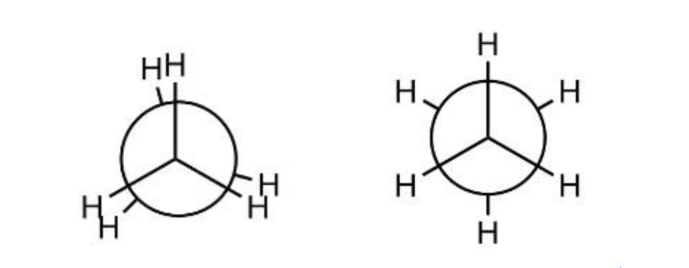
\includegraphics[scale=.7]{../src/img/newmanEthan.png}
    \caption{Newman Darstellung von Ethan}
\end{figure}


Wie man in Abbildung 1 erkennen kann gibt es zwei Extrema, links sind die H-Atome genau hintereinander angeordnet, es kommt somit zu einer größeren
Abstoßung der negativ geladenen $sp^3$-Orbitale. Diese Anordnung nennt sich auch ''eclipsed''. Bei der rechten Darstellung sind die Orbitale weiter
voneinander entfernt, es können daher nicht zu einer so starke elektrostatischen Abstoßung kommen wie bei der Linken. Diese Anordnung nennt sich ''staggerd''.\\
Mit dem Programm HyperChem wurden in der Laboreinheit, die Energieunterschiede zwischen verschieden Diederwinkel bestimmt. Dabei wurden
von jedem Zweierteam sechs semiempirische und zwei ab-initio Methoden verwendet (siehe Abbildung 2 und 3).

\begin{figure}[H]
    \centering
    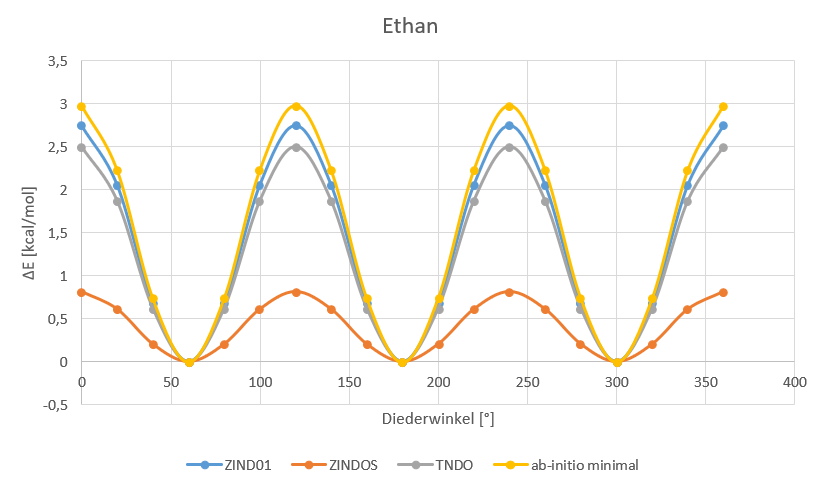
\includegraphics[scale=.7]{../src/img/ethan1.png}
    \caption{Ethan}
\end{figure}

\begin{figure}[H]
    \centering
    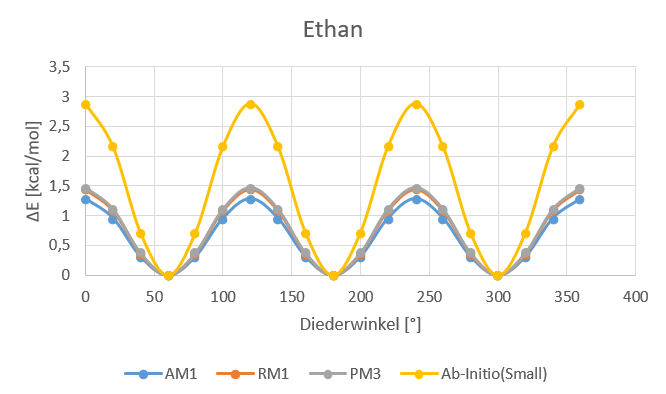
\includegraphics[scale=.9]{../src/img/ethan2.png}
    \caption{Ethan}
\end{figure}

Um alle Graphen auf eine Achse zu skalieren, wurden von allen, mit HyperChem bestimmten Werte für die elektronische Anregung, die geringste
elektronische Anregung subtrahiert. Desweiteren sieht man der Graph je vier Maxima und drei Minima bei einer Umdrehung von 360$^\circ$ hat.
Wenn man bei der linken Anordnung aus Abbildung 1 bei $0^\circ$ anfängt, dann sind die Maxima jeweils bei, $0^\circ$, $120^\circ$, $240^\circ$
und wieder bei $360^\circ$. Die Minima befinden sich bei $60^\circ$, $180^\circ$ und $300^\circ$.\\
Weiter ist noch zu sehen, dass alle Methoden verschiedene Ergebnisse liefern, das liegt an der Tatsache, dass jede Methode für eine bestimmte
Aufgabe optimiert wurde und dann andere Parameter nicht berücksichtigt wurden.

\subsection{Auswertung der erhaltenen Werte}
Um den Energieunterschied zwischen der gestaffelten und der verdeckten Konformation zu bestimmen, müssen folgende Werte bekannt sein:
\begin{itemize}
    \item Die maximale und minimale ZPE (Zero Point Energie).
    \item Die maximale und minimale Energie der elektronischen Anregung.
\end{itemize}
Mit diesen Werten kann über folgende Beziehung bestimmt werden:
\begin{align*}
    \Delta \braket{\tilde{e}}(T) &= \Delta e^V (0) + \Delta e^{el} (0) \\
                                 &= \Delta ZPE + \Delta e^{el}   
\end{align*} 
Damit gilt:
\begin{align}
    \Delta e_{mol} = \Delta ZPE + \Delta e^{el} 
\end{align}
% Table generated by Excel2LaTeX from sheet 'Eingabe'
\begin{table}[H]
  \centering
  \caption{Berechnungen der Energien}
  \begin{tabular}{lrrrrrrr}
    \toprule
    \textbf{Methode} & \multicolumn{1}{l}{\boldmath{}\textbf{$e^{el}_{min}$ [kcal/mol]}\unboldmath{}} & \multicolumn{1}{l}{\boldmath{}\textbf{$ZPE_{min}$}\unboldmath{}} & \multicolumn{1}{l}{\boldmath{}\textbf{$e^{el}_{max}$}\unboldmath{}} & \multicolumn{1}{l}{\boldmath{}\textbf{$ZPE_{max}$}\unboldmath{}} & \multicolumn{1}{l}{\boldmath{}\textbf{$\Delta e_{elec}$}\unboldmath{}} & \multicolumn{1}{l}{\boldmath{}\textbf{$\Delta ZPE$}\unboldmath{}} & \multicolumn{1}{l}{\boldmath{}\textbf{$\Delta e_{mol}$}\unboldmath{}} \\
    \midrule
    \textit{ZIND01} & -1821,792 & 65,930 & -1819,042 & 65,245 & 2,749 & -0,685 & 2,064 \\
    \textit{ZINDOS} & -3491,392 & 64,060 & -3490,575 & 62,859 & 0,818 & -1,201 & -0,383 \\
    \textit{TNDO} & -1842,166 & 65,250 & -1839,666 & 64,564 & 2,500 & -0,686 & 1,814 \\
    \textit{ab-initio minimal} & -49137,871 & 56,280 & -49134,887 & 55,622 & 2,984 & -0,658 & 2,326 \\
    \midrule
    \textit{AM1} & -7821,005 & 46,608 & -7819,756 & 46,112 & 1,249 & -0,496 & 0,753 \\
    \textit{RM1} & -7763,136 & 45,194 & -7761,745 & 44,604 & 1,391 & -0,590 & 0,801 \\
    \textit{PM3} & -7611,633 & 46,476 & -7610,204 & 45,845 & 1,429 & -0,631 & 0,798 \\
    \textit{Ab-Initio(Small)} & -49443,952 & 50,230 & -49440,147 & 49,845 & 3,805 & -0,385 & 3,420 \\
    \midrule
    \midrule
    \textit{Mittelwert} &       &       &       &       & 2,116 & -0,666 & 1,449 \\
    \textit{Stabw.} &       &       &       &       & 1,041 & 0,240 & 1,186 \\
    \textit{Präzision MW.} &       &       &       &       & 0,425 & 0,098 & 0,484 \\
    \bottomrule
    \end{tabular}%
  \label{tab:addlabel}%
\end{table}%


\subsection{Statistische Fehlerrechnung}

Um den Größtfehler von $\Delta e_{mol} = \Delta ZPE + \Delta e^{el} $ zu bestimmen, wird die Gauß'sche Formel zur Fehlervorpflanzung benutzt.

\begin{align}
    f(x, y, ...) = \abs{\frac{\delta f}{\delta x}} \cdot \Delta x + \abs{\frac{\delta f}{\delta y}} \cdot \Delta y + ...
\end{align}

Um die Formel besser lesbar zu machen, wird $\Delta e_{mol}$ mit f(x, y) ersetzt.

\begin{align*}
    f(x, y) =  \abs{\frac{\delta (x + y)}{\delta x}} \cdot \Delta x + \abs{\frac{\delta (x + y)}{\delta y}} \cdot \Delta y = \Delta x + \Delta y 
    = \pm 1.281 \, [kcal/mol]
\end{align*}

\subsection{Vergleich der Methoden}

Die ZINDOS Methode ist für unsere Fragestellung nicht brauchbar, da dass Ergebnis darauf schließen lässt, dass die Energie der gestaffelten Konformation
höher ist als in der Verdeckten. Dieses Ergebnis wiederspricht den physikalischen Grundlagen dieses Versuches. 

\subsection{Bestimmung des Schwingungsspektrum}
Zur Bestimmung der Schwingungsspektren wurden drei Schwingungsarten bei verschiedenen Wellenzahlen notiert.

\begin{table}[H]
    \centering
    \begin{tabular}{cl}
        \toprule 
        Wellenzahl [$cm^{-1}$] & Schwingungsart \\
        \midrule
        275,1	& Drehschwingung der Methylgruppe \\
        1369,2	& Asymmetrische C-H Streckschwingung \\
        2121,7	& Symmetrische Streckschwingung  \\
        \bottomrule
    \end{tabular}
\end{table}
Ausgehend von der Wellenzahl wird die Wellenlänge wie folgend berechnet:
\begin{align}
    \lambda = \frac{1}{Wellenzahl} \cdot 10^7
\end{align}

Die Energie wird über die Planck-Einstein-Korrelation berechnet:
\begin{align}
    E = \frac{hc}{\lambda}
\end{align}

\begin{table}[H]
    \centering
    \begin{tabular}{ll}
        $h...Plancksches Wirkungsquantum \, [J/s]$ & $c...Lichtgeschwindigkeit \, [m/s]$ \\
        $\lambda...Wellenlänge \, [m]$ &  \\
    \end{tabular}
\end{table}

Die Temperatur wird dann schließlich mit folgender Formel berechnet:
\begin{align*}
    \Delta E = k_b T \\
    T = \frac{\Delta E}{k_b}
\end{align*}
% Table generated by Excel2LaTeX from sheet 'Tabelle1'
\begin{table}[H]
  \centering
  \caption{Add caption}
    \begin{tabular}{clrrr}
    \toprule
    \multicolumn{1}{l}{\textbf{Wellenzahl [1/cm]}} & \textbf{Schwingungsart} & \multicolumn{1}{l}{\boldmath{}\textbf{$\lambda$ [nm]}\unboldmath{}} & \multicolumn{1}{l}{\boldmath{}\textbf{$\Delta E$ J}\unboldmath{}} & \multicolumn{1}{l}{\textbf{Temp. [K]}} \\
    \midrule
    275,1 & Drehschwingung der Methylgruppe & 36350,42 & 5,46E-21 & 395,81 \\
    1369,2 & Asymmetrische C-H Streckschwingung & 7303,53 & 2,72E-20 & 1969,97 \\
    2121,7 & Symmetrische Streckschwingung & 4713,2 & 4,21E-20 & 3052,65 \\
    \bottomrule
    \end{tabular}%
  \label{tab:addlabel}%
\end{table}%


\subsection{Bestimmung Bestzungszahlen}

Um auf die Besetzungszahl zu kommen wird ein Energiedifferenzwert gewählt an dem die Berechnung durchgeführt wird und eine Temperatur. Die Besetzungszahl gibt das Verhältnis zwischen den Molekülen die bei dieser Temperatur den angeregten Energiezustand und denen die den Ausgangszustand besetzen.
In diesem Fall wird mit der Energie der Drehschwingung der Methylgruppe und den Temperaturen: $\approx$0K, 293,15 K und 473,15 K gerechnet.
Die Formel zur Berechnung lautet:
\begin{align}
    n_i = \frac{N_i}{N_0} = e^{\frac{-\Delta E}{k_b T}}
\end{align}

% Table generated by Excel2LaTeX from sheet 'Tabelle1'
\begin{table}[htbp]
  \centering
  \caption{Add caption}
    \begin{tabular}{lccc}
    \toprule
    \textbf{T [K]} & \multicolumn{1}{l}{\boldmath{}\textbf{$\approx 0$K}\unboldmath{}} & \multicolumn{1}{l}{\textbf{293.15K}} & \multicolumn{1}{l}{\textbf{473.15K}} \\
    \midrule
    \textit{Bestzungszahl 1} & 0     & 2,59E-01 & 4,33E-01 \\
    \textit{Bestzungszahl 2} & 0     & 1,20E-03 & 1,55E-02 \\
    \textit{Bestzungszahl 3} & 0     & 3,02E-05 & 1,58E-03 \\
    \bottomrule
    \end{tabular}%
  \label{tab:addlabel}%
\end{table}%

\subsection{Berechnung der Geschwindigkeitskonstante der Rotation}

Die Geschwindigkeitskonstante gibt hier an, in welcher Geschwindigkeit das Molekül zwischen den Zuständen fluktuiert. \\
Der $\Delta G$-Wert von Ethan wurde bestimmt, indem die Differenz zwischen Maximum und Minimum der Freien Gibbschen Enthalphie bei 293,15 K gebildet wird.
\begin{align*}
    \Delta G = (-7714.95 - -7715.74) kcal/mol = 0.79 kcal/mol = 3.305 kJ/mol  
\end{align*}
Daraus lässt sich nun aus dieser Formel die Geschwindigkeitskonstante bestimmen:
\begin{align}
    K = \frac{k_b T}{h} \cdot e^{\frac{- \Delta G}{RT}}
\end{align}

Daraus folgt durch einsetzen: $K = 1.57 \cdot 10^{-12} s^{-1}$
